\documentclass[a4paper, 12pt]{article} %[optional paper size, landscape]
\usepackage[utf8]{inputenc}

% Mount the package to be used.
\usepackage{graphicx} % thumbs, dollars...
\usepackage{url}
\usepackage[margin = 2cm]{geometry}

\usepackage[bottom]{footmisc}
\usepackage{marvosym} % for Batman symbol
\usepackage{wasysym}
\usepackage{hyperref}
\usepackage{natbib}
\usepackage{amsmath}

\title{Latex Introduction - Devil Ray }
\author{Viktor Chao}
\date{June 2018}

\begin{document}

\maketitle
\tableofcontents

\vspace{3cm}
This space is intentionally left blank.

\newpage

\section{Introduction}
\subsection{ordered}
this section, we'll take a look at the powerful tool - Latex.
hello world! Without section command, there will be no indented feature in the begin of the paragraph.

\subsection{unordered}
Here is some text it is the first paragraph of my document. Second sentence follows the first.

I'm writing on line 13, bit it's on the same line.\\
Here is a new line. % This is a comment, it will not be printed.

Leaving a blank line starts a new paragraph w/ indented feature. \cite{maxwell1992thermodynamics}

\vspace{1cm}

\section{Key-Takeaways}

Access this document online: \url{https://v2.overleaf.com/read/pnfhvvbbzxfc}
Or access it by clicking \href{https://v2.overleaf.com/read/pnfhvvbbzxfc}{here}.

\begin{itemize}
    \item Extra spaces      do not appear. \\
        Start typing after tabs.
    \item Insert and re-scale a image.

        \begin{figure}[ht] % ht: here, top
        \centering
        \includegraphics[width=8cm,height=5 cm]{DevilRay.JPG} % try  Scale the picture with [scale = 0.4][width=\textwidth]
        \caption{Look! I can fly.}
        \label{fig:my_DevilRay}
        \end{figure}

        Here is some text after my image.
    \item un-ordered shopping-list

        \begin{itemize}
            \item milk,
            \item banana,
            \item soap,
        \end{itemize}  
    
    \item ordered list:
        \begin{enumerate}
            \item chocolate,
            \item soap,
                \begin{enumerate}
                    \item must be bar soap,
                    \item prefer Dove brand.
                \end{enumerate}
            \item milk.
    \end{enumerate}
    
    \item Why the Devil-Ray is the best choice? 
    \footnote{9 Facts About Devil Rays - \url{http://www2.padi.com/blog/2015/10/31/9-facts-about-devil-rays/}}
 
    \begin{itemize}
    

 
        \item they have been around for 20-25 million years.
        
        \item the deepest, fastest divers in the ocean. (Devil rays can dive to depths of nearly 2km for around 60-90 minutes, at speeds of 13mph or 22km/h.)
        
        \item Devil rays are actually harmless, shy creatures and filter-feed on...
        
        \begin{enumerate}
            \item plankton,
            \item krill,
            \item small fish.
            
        \end{enumerate}
    \end{itemize}
    
    \item Formatting
    \begin{flushright} This text is right justified.
    \end{flushright}
    \begin{center} Centered text.
    \end{center}

Return to paragraph mode.

Here is some \textbf{bold text}.\\
Now for some \textit{italic font}.\\
\emph{Here is some  \emph{emphasized text.}}

This is {\large a bit larger} text.\\
Slightly {\Large bigger} text.\\
Even {\LARGE bigger} again.\\
Now for some {\small small} text.

    \item Keep typing on the next page.
    
    \item Symbols
    
    There is a 40\% chance of rain today.
    I like cats \& dogs.\\
    To type backslash using a special command: \textbackslash 
    
    Batman symbol: \Bat
    
    My friend's name is \AA Shild. \cite{mittelbach2004latex}
    
{\Huge    We are learning \LaTeX}

    \item Tables

\vspace{1cm}
    
    \item Math-modes
    
    \item Citation and Reference
    
\end{itemize}

    \pagebreak

\section{Tables}

Let's look at some tables now.

\begin{table}[ht]
    \centering
    \caption{My first table}
    \begin{tabular}{|p{0.1\textwidth}|cr|}
    % cr: centered, round. | for vertical-lines.
        \hline
        really long column name & column 2 & column 3 \\
        1 &  &  \\ % "&" for allignment
        \hline
        a & b & c\\
        d & e & f\\
        \hline
    \end{tabular}
    \label{tab:my_label}
\end{table}

% Generate table from .csv files:  https://www.tablesgenerator.com/

    
%\begin{figure}[ht] % ht: here, top

Refer to \autoref{fig:my_Wallpaper}

        \centering
        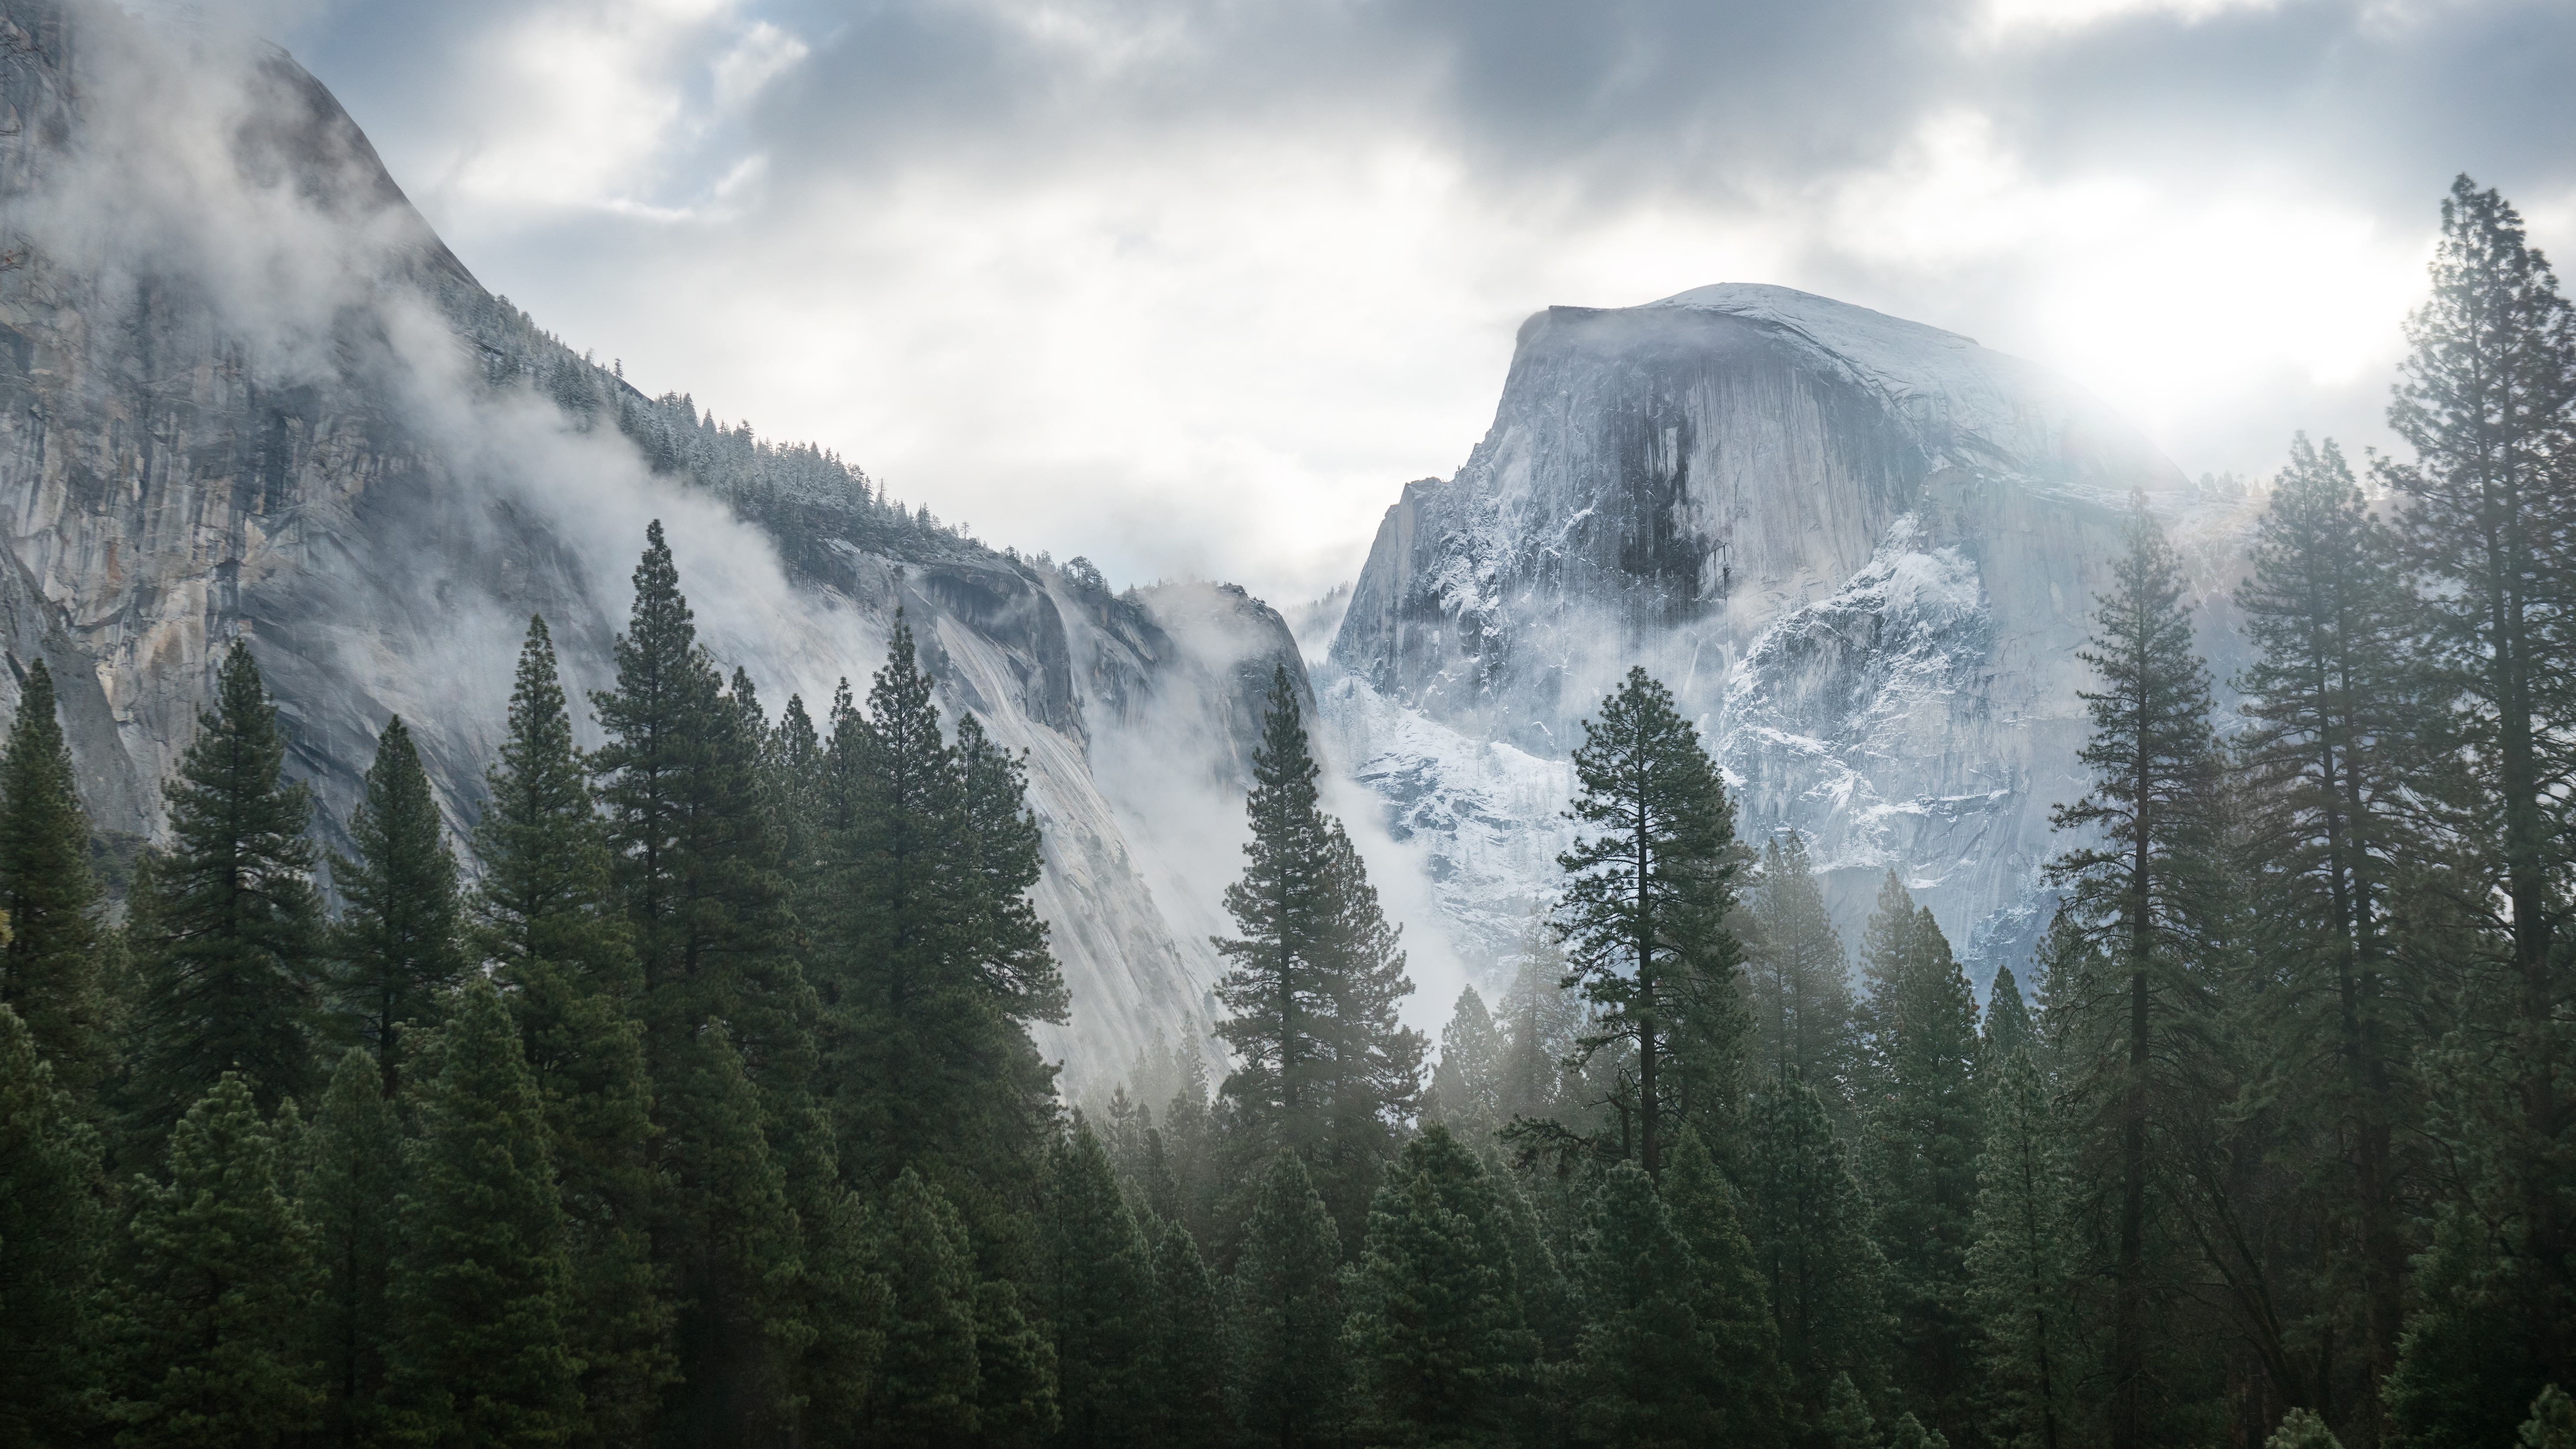
\includegraphics[scale = 0.2]{Wallpaper.jpg}
        \caption{Wallpaper is fancy.}
        \label{fig:my_Wallpaper}
\end{figure}
\section{Mathematics}

Dollar signs are used to type mathematics:
$e^{i\pi}+1=0$.

Display mathematics:
$$
e^{i\pi}+1=0.
$$   \cite{9783639174304}

% the align environment (package: amsmath, amssymb)
Aligned mathematics:
\begin{align}
    e^{i\pi}&=\cos(\pi)+i\sin(\pi)\\
    &= -1 % "&" is used for alignment.
\end{align}

Aligned mathematics w/o number:
\begin{align*}
    e^{i\pi}&=\cos(\pi)+i\sin(\pi)\\
    &= -1 % "&" is used for alignment.    
\end{align*}

\section{Challenges}

\begin{itemize}
    \item Formatting and symbols challenge.
    \begin{center}
        {\Large ``Devil Rays"} are \textit {the {\textbf{best!}}} {\Smiley} {\frownie}
        %\RightThumbsUp
\end{center}

    \item Math-mode
$$
\sin(\frac{\pi}3)=\frac{\sqrt{3}}2
$$

\end{itemize}


%\input{bibliography.bib}

\newpage
\bibliographystyle{plain}
\bibliography{bibliography.bib}

\end{document}
